To add a second chapter, simply include it in the main document.

\section{General structure}
\subsection{JModelica(Compile)Phase}
The JModelica environment is used to compile the Modelica models to JModelicas JMU representation \cite{jmodelicaorg}\nocite{*}. This representation is internally represented as a, possibly nonlinear, DAE. Since ProMoVis assumes the systems to be linear, the compiled model needs to be linearised around an operating point. Here an assumption is made, that the model is stable at Time 0. See Appendix \ref{appA} for a complete overview of the prerequisites for the original model.\\\\After linearisation a DAE on the following form can be extracted:
\begin{equation}
E*dx = A*x + B*u + F*w + g
\end{equation}
This represenation should be familiar, the x and dx vectors represents the states and outputs of the linearized system. The u vector represents declared inputs, w is algebraic varibles, that is all variables in the system that has no derivative declared.Finally g is a constant bias.\\\\The linearization also outputs some useful information that we later use in the generation of ProMoVis scenarios:
\begin{itemize}
\item \textit{State names}, corresponding to the declared variable names from the original Modelica file.
\item \textit{Input names}, corresponding to the declared input names from the original Modelica file.
\item \textit{Algebraic names}, corresponding to the declared algebraic variable names from the original Modelica file.
\item \textit{Operating points} for the linear model \textit{dx0},\textit{w0}, \textit{u0} and \textit{x0}. Which is , in later stages, used to provide feedback for the user regarding the validity of the resulting model.
\end{itemize}
From now on we will refer to states and algebraic variables as simply "variables" and whenever a distinction between the two is needed, it will be explicitly declared. When the DAE is obtained, the task is then to extract the relations between the variables and in the DAE.

\subsection{Generation of the internal structure}
The generation of the internal structure is best illustrated with the following example.\\\newline
When the linearised model is extracted and we have all non-zero diagonal elements the system might be represented as:\\\newline
$
\begin{bmatrix} E_{11} & E_{12} \\ E_{21} & E_{22} \\ E_{31} & E_{32} \\ E_{41} & E_{42} \end{bmatrix} \left[ \begin{array}{c} x0' \\ x1' \end{array} \right]
= \begin{bmatrix} A_{11} & A_{12} \\ A_{21} & A_{22} \\ A_{31} & A_{32} \\ A_{41} & A_{42} \end{bmatrix} \times \left[ \begin{array}{c} x0 \\ x1 \end{array} \right] + \begin{bmatrix} B_{11} & B_{12} \\ B_{21} & B_{22} \\ B_{31} & B_{32} \\ B_{41} & B_{42} \end{bmatrix} \times \left[ \begin{array}{c} u0 \\ u1 \end{array} \right]+
\begin{bmatrix} F_{11} & F_{12} \\ F_{21} & F_{22} \\ F_{31} & F_{32} \\ F_{41} & F_{42}\end{bmatrix} \times \left[ \begin{array}{c} w0 \\ w1 \end{array} \right]$

The task is now, to find which of the rows in the system that should be solved for which variable so that the whole system can be solved. A demand on the system is that it should not contain any Algebraic loops. For a more thorough discussion regarding this please review Appendix \ref{appB}\\\\After retrieving which row that we should solve for which of the variables we build up an intermediate representation of the SFG where we store each of the variables together with all of its input dependencies.\\\\
As an example, if we assume that we should solve row 1 for x0 we get the following:\\\\$\begin{array}{rcl} E_{11}*x0*s  +E_{12}*x1*s=A_{11}*x0  +A_{12}*x1 +B_{11}*u0  +B_{12}*u1  +F_{11}*w0  +F_{12}*w1 \end{array}$\\
\\Putting x0 alone on the left-hand side and collecting the coefficients then yields:\\\\$\begin{array}{rcl} (E_{11}*s-A_{11})*x0  =(A_{12}-E_{12}*s)*x1 +B_{11}*u0  +B_{12}*u1 +F_{11}*w0  +F_{12}*w1 \end{array}$\\\\
Finally, solving for x0 yields:\\\\
$\begin{array}{rcl} x0  = \frac{(A_{12}-E_{12}*s)}{(E_{11}*s-A_{11})}*x1 +\frac{B_{11}}{(E_{11}*s-A_{11})}*u0  +\frac{B_{12}}{(E_{11}*s-A_{11})}*u1 ++\frac{F_{11}}{(E_{11}*s-A_{11})}*w0 +\frac{F_{12}}{(E_{11}*s-A_{11})}*w1\end{array}$\\\newline Which would correspond to the following SFG:\\Internally we then represent each of the variables in the following form.\\\newline
%

\setlength\fboxsep{0pt}
\setlength\fboxrule{0.5pt}
\fbox{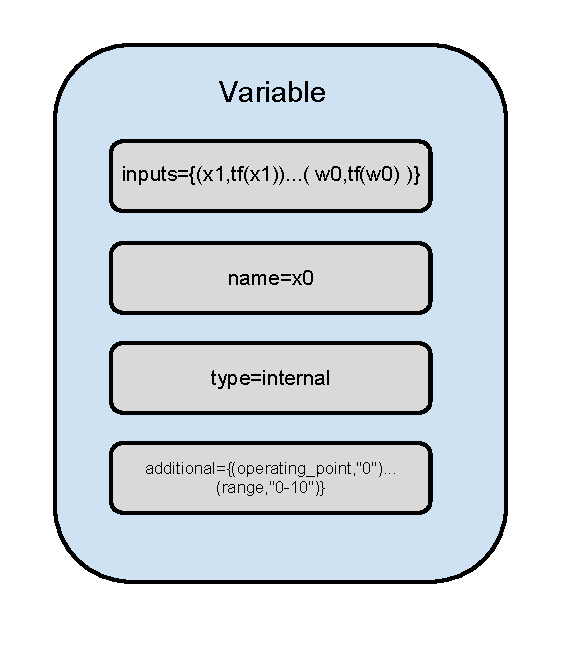
\includegraphics[scale=0.8,bb=0 0 97mm 111mm] {Figures/variable_structure.pdf}}\\\newline Here "inputs" is a dictionary with variable names as keys and the corresponding transfer functions as a values. A transfer function, in the export tool,is using the same convention as in MatLab to represent the numerator and denominator coefficients for a transfer function in two separate arrays. It also has some methods, described later, that are used in the generations of the ProMoVis specific structure. 


\subsection{Validation and Transformations}
\subsection{Scenario generation}

\section{Interfacing with the tool}
\section{Important design choices}
\section{A small case study}